\subsection{Rollator}
\noindent The most clear option for the choice of walker frame, to be outfitted with motors and the electronics system, is a standard medical rollator, available on common online commercial marketplaces. The steel frame remains at a weight under 20 pounds, and its dimensions are given as 25.5"D x 31"W x 23.5"H. It comes with a seat, storage compartment, and pneumatically actuated brakes. The FORWARD team plans to remove the seat and storage compartment to replace with the electronics housing, change the braking system to velocity control, and to dismount the wheels to install the DC motors. The wheels are also 7.5 inch diameter, which we anticipate will provide enough torque for the adaptive velocity control and steering enacted by the motor shield.\\

\begin{figure}[H]
	\centering
	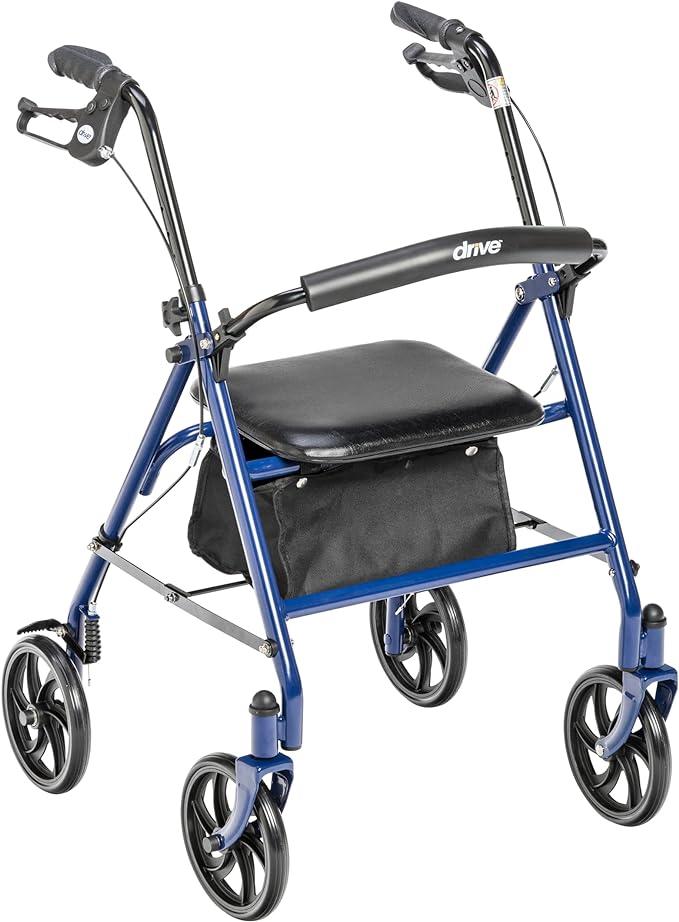
\includegraphics[width=0.3\textwidth]{./Images/rollator-amaz.jpg}
	\caption{\label{fig:rollator-amaz}Medical Rollator}
\end{figure}

\noindent There are many other variants of rollators available - some with enlarged front wheels and some with only three wheels altogether. There seem to be two main shapes of frame: A and what we can call $\lambda$. We estimate that, the A frame is more appropriate for our purposes. FORWARD velocity control and electric braking also requires four wheels.\\

% matthew
\subsection{Electronics Chassis}
\noindent Discuss psychical location of all elements and components on the walker frame and explain the reason. explain plans for wiring and attachment (tape, glue, screws etc).\\

\noindent discuss positioning of sensors on the walker, wiring; need for IMU to be level. installation of haptics. implementation of earpiece being available to user. braking, motor speed control. physical object avoidance margins. obstacle classifications.\\

\noindent sensor housing, surface mount IMU (on PCB), surface mount LiDAR? (on PCB), PCB centrally mounted, bluetooth module centrally mounted?\\

\noindent headlights? steering? braking? curb assist? tipover prevention with motors explained\\